\documentclass[
11pt, % The default document font size, options: 10pt, 11pt, 12pt
codirector, % Uncomment to add a codirector to the title page
]{charter}

% El títulos de la memoria, se usa en la carátula y se puede usar el cualquier lugar del documento con el comando \ttitle
\titulo{Controlador de pH para cultivos hidropónicos}

% Nombre del posgrado, se usa en la carátula y se puede usar el cualquier lugar del documento con el comando \degreename
\posgrado{Carrera de Especialización en Sistemas Embebidos} 
%\posgrado{Carrera de Especialización en Internet de las Cosas} 
%\posgrado{Carrera de Especialización en Inteligencia Artificial}
%\posgrado{Maestría en Sistemas Embebidos} 
%\posgrado{Maestría en Internet de las cosas}
% IMPORTANTE: no omitir titulaciones ni tildación en los nombres, también se recomienda escribir los nombres completos (tal cual los tienen en su documento)
% Tu nombre, se puede usar el cualquier lugar del documento con el comando \authorname
\autor{Ing. Iván Podoroska}

% El nombre del director y co-director, se puede usar el cualquier lugar del documento con el comando \supname y \cosupname y \pertesupname y \pertecosupname
\director{Ing. Juan Pepito}
\pertenenciaDirector{pertenencia} 
\codirector{} % para que aparezca en la portada se debe descomentar la opción codirector en los parámetros de documentclass
\pertenenciaCoDirector{}

% Nombre del cliente, quien va a aprobar los resultados del proyecto, se puede usar con el comando \clientename y \empclientename
\cliente{Francisco Yuvone}
\empresaCliente{Cannfeel SA}
 
\fechaINICIO{29 de abril de 2024}		%Fecha de inicio de la cursada de GdP \fechaInicioName
\fechaFINALPlan{11 de junio de 2024} 	%Fecha de final de cursada de GdP
\fechaFINALTrabajo{10 de diciembre de 2024}	%Fecha de defensa pública del trabajo final


\begin{document}

\maketitle
\thispagestyle{empty}
\pagebreak


\thispagestyle{empty}
{\setlength{\parskip}{0pt}
\tableofcontents{}
}
\pagebreak

\section*{Registros de cambios}
\label{sec:registro}


\begin{table}[ht]
\label{tab:registro}
\centering
\begin{tabularx}{\linewidth}{@{}|c|X|c|@{}}
\hline
\rowcolor[HTML]{C0C0C0} 
Revisión & \multicolumn{1}{c|}{\cellcolor[HTML]{C0C0C0}Detalles de los cambios realizados} & Fecha      \\ \hline
0      & Creación del documento                                 &\fechaInicioName \\ \hline
1      & Se completa hasta el punto 5 inclusive                 & {7} de {mayo} de 2024 \\ \hline
2      & Se completa hasta el punto 9 inclusive					& {14} de {mayo} de 2024 \\ \hline
3      & Se completa hasta el punto 12 inclusive                & {21} de {mayo} de 2024 \\ \hline
%4      & Se completa el plan	                                 & {día} de {mes} de 202X \\ \hline
%		  Se puede agregar algo más \newline
%		  En distintas líneas \newline
%		  Así                                                    & {día} de {mes} de 202X \\ \hline

% Si hay más correcciones pasada la versión 4 también se deben especificar acá

\end{tabularx}
\end{table}

\pagebreak



\section*{Acta de constitución del proyecto}
\label{sec:acta}

\begin{flushright}
Buenos Aires, \fechaInicioName
\end{flushright}

\vspace{2cm}

Por medio de la presente se acuerda con el Ing. \authorname\hspace{1px} que su Trabajo Final de la \degreename\hspace{1px} se titulará ``\ttitle'' y consistirá en la implementación de un prototipo de un sistema de control de pH para cultivos hidropónicos. El trabajo tendrá un presupuesto preliminar estimado de 720 horas y un costo de \$14510000, con fecha de inicio el \fechaInicioName\hspace{1px} y fecha de presentación pública el \fechaFinalName.

Se adjunta a esta acta la planificación inicial.

\vfill

% Esta parte se construye sola con la información que hayan cargado en el preámbulo del documento y no debe modificarla
\begin{table}[ht]
\centering
\begin{tabular}{ccc}
\begin{tabular}[c]{@{}c@{}}Dr. Ing. Ariel Lutenberg \\ Director posgrado FIUBA\end{tabular} & \hspace{2cm} & \begin{tabular}[c]{@{}c@{}}\clientename \\ \empclientename \end{tabular} \vspace{2.5cm} \\ 
\multicolumn{3}{c}{\begin{tabular}[c]{@{}c@{}} \supname \\ Director del Trabajo Final\end{tabular}} \vspace{2.5cm} \\
\end{tabular}
\end{table}




\section{1. Descripción técnica-conceptual del proyecto a realizar}
\label{sec:descripcion}

La agricultura hidropónica es un método utilizado para cultivar plantas sin tierra, usando una solución rica en nutrientes. Mediante el contacto directo de las raíces con la solución nutritiva se logra un suministro constante y eficiente de macronutrientes y micronutrientes esenciales. Para su absorción, intervienen procesos de transporte activo y ósmosis, que requieren un pH controlado para garantizar el transporte de los nutrientes hacia la planta.

La empresa Cannfeel incorpora equipos para la medición y control de cultivos de precisión mediante Internet de las Cosas (IOT, por sus siglas en inglés). El objetivo de este proyecto es sumar un producto más al ecosistema, que sea capaz de regular y controlar el pH de soluciones nutritivas. Deberá poder integrarse a los equipos existentes y funcionar de manera autónoma.

El proyecto permitirá abstraer al cultivador de la tarea manual de la regulación del pH de la solución nutritiva. Al estar incluida en el ecosistema de la empresa, el usuario podrá tener acceso en tiempo real al estado de la solución nutritiva a través de una aplicación web ya implementada.

El sistema deberá ser capaz de medir el pH y la temperatura de una solución nutritiva. Contará con un \textit{encoder} rotativo con botón y una pantalla, donde el usuario podrá ingresar el valor de pH que desee para la solución. El sistema tendrá que ser capaz de controlar el pH, utilizando una solución \textit{buffer}. Para llevar a cabo la inyección de la sustancia reguladora, se contará con una bomba peristáltica como se observa en la figura \ref{fig:diagBloq}.

El reto del presente proyecto es poder implementar tanto el hardware como el firmware asociado para alcanzar la solución propuesta en el tiempo estimado.

En la figura \ref{fig:diagBloq} se representa el diagrama en bloques del sistema.

\begin{figure}[htpb]
\centering 
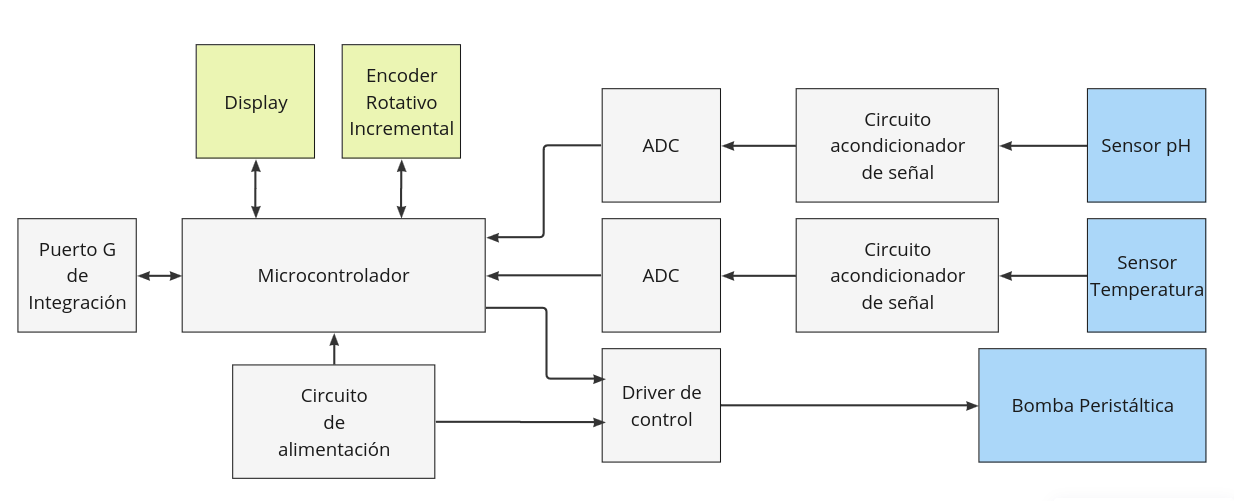
\includegraphics[width=.85\textwidth]{./Figuras/diagBloq.png}
\caption{Diagrama en bloques del sistema.}
\label{fig:diagBloq}
\end{figure}

En la figura \ref{fig:diagCtrl} se representa el diagrama en bloque del esquema de control a implementar.

\begin{figure}[htpb]
\centering
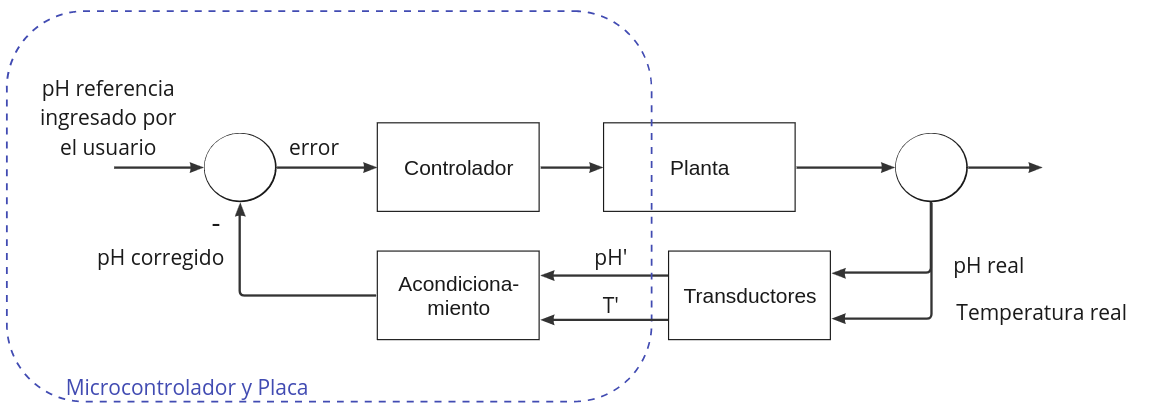
\includegraphics[width=.85\textwidth]{./Figuras/diagCtrl.png}
\caption{Diagrama de control del sistema.}
\label{fig:diagCtrl}
\end{figure}


\section{2. Identificación y análisis de los interesados}
\label{sec:interesados}

\begin{table}[ht]
%\caption{Identificación de los interesados}
%\label{tab:interesados}
\begin{tabularx}{\linewidth}{@{}|l|X|X|l|@{}}
\hline
\rowcolor[HTML]{C0C0C0} 
Rol           & Nombre y Apellido & Organización 	& Puesto 	\\ \hline
%Auspiciante   &                   &              	&        	\\ \hline
Cliente       & \clientename      &\empclientename	& CTO      	\\ \hline
%Impulsor      &                   &              	&        	\\ \hline
Responsable   & \authorname       & FIUBA        	& Alumno 	\\ \hline
%Colaboradores &                   &              	&        	\\ \hline
Orientador    & \supname	      & \pertesupname 	& Director del Trabajo Final \\ \hline
%Equipo        & miembro1 \newline 
%				miembro2          &              	&        	\\ \hline
%Opositores    &                   &              	&        	\\ \hline
%Usuario final &                   &              	&        	\\ \hline
\end{tabularx}
\end{table}

\section{3. Propósito del proyecto}
\label{sec:proposito}

Desarrollar un prototipo funcional capaz de medir y controlar en línea el pH de una solución nutritiva para cultivos hidropónicos. Se busca que el cultivador no deba realizar de manera manual esta tarea.

\section{4. Alcance del proyecto}
\label{sec:alcance}

El presente proyecto incluye:
\begin{itemize}
	\item Diseño e implementación de un prototipo.
		\begin{itemize}
		\item Diseño de hardware.
		\item Diseño de firmware.
		\end{itemize}
	\item Elección del display para la interfaz.
	\item Elección del \textit{encoder} rotativo.
	\item Elección del sensor de pH.
	\item Elección del método de sensado de temperatura.
		\begin{itemize}
		\item Elección del sensor de temperatura.
		\end{itemize}
	\item Elección de la bomba peristáltica.
	\item Ensayos de funcionamiento en campo.
\end{itemize}

El presente proyecto no incluye:
\begin{itemize}
	\item Diseño y fabricación de la carcaza del dispositivo.
	\item Modificaciones en la aplicación web existente.
	\item Manual de usuario.
	\item Manual de instalación.
\end{itemize}


\section{5. Supuestos del proyecto}
\label{sec:supuestos}


\begin{itemize}
	\item Se tendrá a disposición los equipos de la empresa Cannfeel SA cuando sean requeridos.
	\item Se utilizarán herramientas que no requieran licencia.
	\item Todos los componentes estarán disponibles para su compra.
	\item Será posible desarrollar los PCBs del prototipo de prueba.
	\item Los tiempos de importación y de fabricación estarán dentro de lo planeado.
	\item No habrá problemas para la importación de lo requerido.
	\item El presupuesto no superará en gran medida a lo estimado.
\end{itemize}


\section{6. Requerimientos}
\label{sec:requerimientos}

\begin{enumerate}
	\item Requerimientos técnicos
		\begin{enumerate}
			\item El sistema se deberá alimentar con una fuente de alimentación externa.
			\item El hardware deberá tener un driver para manejar una bomba peristáltica.
			\item El hardware deberá contar con un conector para una sonda de pH.
			\item El hardware deberá contar con un conector para una sonda de temperatura.
			\item El hardware deberá acondicionar la señal de la sonda de pH.
			\item El hardware deberá acondicionar la señal de la sonda de temperatura.
			\item El sistema deberá encender y apagar una bomba de recirculación opcional.
		\end{enumerate}
		
	\item Requerimientos funcionales
		\begin{enumerate}
			\item El sistema deberá compensar la medición de pH con la temperatura de la solución.
			\item El sistema deberá reconocer una falla por falta de solución \textit{buffer}.
			\item El sistema deberá reconocer si no puede controlar el pH de la solución nutritiva.
			\item El sistema deberá tener un modo de control donde intente corregir el pH de la solución constantemente.
			\item El sistema deberá contar con un modo de solo lectura que se limite a mostrar en la pantalla los valores obtenidos de los sensores.
			\item El sistema deberá contar con un modo de configuración donde se podrán calibrar los sensores y configurar el valor deseado de pH para el control.
		\end{enumerate}
		
	\item Requerimientos de interoperabilidad
		\begin{enumerate}
			\item El controlador se deberá integrar al ecosistema de dispositivos de la empresa Cannfeel mediante un protocolo propietario.
		\end{enumerate}	
		
	\item Requerimientos de la interfaz
		\begin{enumerate}
			\item El hardware deberá contar con una pantalla no táctil.
			\item El hardware deberá contar con un \textit{encoder} rotativo incremental con botón.
			\item El sistema permitirá configurar los parámetros del controlador desde la interfaz local.
			\item El usuario deberá poder calibrar la sonda de pH en tres puntos desde la interfaz local.
			\item El usuario deberá poder calibrar la sonda de temperatura desde la interfaz local.
		\end{enumerate}
		
	\item Requerimientos de pruebas
		\begin{enumerate}
			\item El sistema no deberá funcionar en modo de regulación si detecta la falta de solución \textit{buffer}.
		\end{enumerate}
		
	\item Requerimientos de documentación
		\begin{enumerate}
			\item Se confeccionarán informes de avance dirigidos al cliente y al director con la finalidad de controlar el avance del proyecto.
			\item Se confeccionará una memoria técnica al finalizar el proyecto.
		\end{enumerate}
\end{enumerate}

\section{7. Historias de usuarios (\textit{Product backlog})}
\label{sec:backlog}

En esta sección se mostrarán las historias de usuarios según los roles de: cliente, usuario final y desarrollador. Se valoraron de acuerdo a un sistema de \textit{story points} basado en la estimación de tres categorías:

\begin{itemize}
	\item Complejidad del trabajo (C):
	\begin{itemize}
		\item Bajo: 1
		\item Medio: 5
		\item Alto: 13		
	\end{itemize}
	\item Dificultad del trabajo (D):
	\begin{itemize}
		\item Bajo: 1
		\item Medio: 3
		\item Alto: 5		
	\end{itemize}
	\item Riesgo del trabajo (R):
	\begin{itemize}
		\item Bajo: 1
		\item Medio: 3
		\item Alto: 5		
	\end{itemize}
\end{itemize}

Para obtener la estimación final, se sumaron los valores asignados a cada aspecto y se aproximaron
al siguiente número de la serie de Fibonacci. Por ejemplo, si la complejidad del trabajo es media (5), la dificultad es alta (5) y la incertidumbre es media (3), las suma de los \textit{story points} es 13 y se aproxima al siguiente número de Fibonacci, que es 21. La valoración final será 21.

\begin{enumerate}
	\item Como cliente, quiero que el sistema sea capaz de comunicarse con otros dispositivos del ecosistema de la empresa para que se integren y mejoren la solución ofrecida. 
	\begin{itemize}
		\item \textit{Story points}: 8 (C:1, D:5, R:1).	
	\end{itemize}
	
	\item Como usuario final, quiero modificar los parámetros de medición del sensor de pH con el objetivo de calibrarlo.
	\begin{itemize}
		\item \textit{Story points}: 3 (C:1, D:1, R:1).	
	\end{itemize}
	
	\item Como usuario final, quiero poder configurar el valor de pH a controlar de manera local para no depender de la conexión a una plataforma. 
	\begin{itemize}
		\item \textit{Story points}: 21 (C:13, D:3, R:3).	
	\end{itemize}
	
	\item Como desarrollador, quiero implementar un controlador de pH preciso y de bajo costo para poder controlar la absorción de nutrientes de las plantas en cultivos hidropónicos.
	\begin{itemize}
		\item \textit{Story points}: 21 (C:13, D:5, R:3).	
	\end{itemize}
\end{enumerate}

\section{8. Entregables principales del proyecto}
\label{sec:entregables}

Los entregables de proyecto son:

\begin{itemize}
	\item Prototipo funcional.
	\item Archivos para la producción del PCB.
	\item Diagrama de circuitos esquemáticos.
	\item Lista de materiales (BOM, por sus siglas en inglés).
	\item Código fuente del firmware.
	\item Informes de avance.
	\item Memoria del trabajo final.
\end{itemize}

\section{9. Desglose del trabajo en tareas}
\label{sec:wbs}

\begin{enumerate}
\item Investigación y documentación (92 h)
	\begin{enumerate}
	\item Investigar sobre el estado del arte (8 h).
	\item Armar el plan de proyecto (32 h).
	\item Investigación y elección de sensor de pH (16 h).
	\item Investigación y elección de sensor de temperatura (16 h).
	\item Investigación y elección de pantalla (12 h).
	\item Investigación y elección de \textit{encoder} rotativo incremental (8 h).
	\end{enumerate}
	
\item Diseño general (36 h)
	\begin{enumerate}
	\item Diseño de diagrama de módulos (8 h).
	\item Diseño de diagrama de conexiones (8 h).
	\item Elección de la fuente de alimentación externa (4 h).
	\item Diseño de las interfaces de la pantalla (16 h).
	\end{enumerate}
	
\item Desarrollo del hardware (152 h)
	\begin{enumerate}
	\item Elección de conectores y componentes de potencia (24 h).
	\item Selección de componentes varios (8 h).
	\item Diseño de diagramas esquemáticos (60 h).
	\item Diseño del PCB y de los archivos de fabricación (40 h).
	\item Armado del prototipo (20 h).
	\end{enumerate}
	
\item Desarrollo del firmware (268 h)
	\begin{enumerate}
	\item Elección de la arquitectura (16 h).
	\item Diseño en papel de los módulos a implementar (12 h).
	\item Diseño de las máquinas de estados (40 h).
	\item Diseño de pruebas (40 h).
	\item Programación de firmware (120 h).
	\item Verificación y validación (40 h).
	\end{enumerate}
	
\item Pruebas y calibración (80 h)
	\begin{enumerate}
	\item Prueba del prototipo en modo de funcionamiento normal (40 h).
	\item Prueba del prototipo en modo de funcionamiento en falla (20 h).
	\item Ajustes finales y puesta a punto (20 h).
	\end{enumerate}
	
\item Presentación final (92 h)
	\begin{enumerate}
	\item Redacción del informe de avances (12 h)
	\item Redacción de la memoria técnica (60 h).
	\item Presentación final (20 h).
	\end{enumerate}
\end{enumerate}

Cantidad total de horas: 720 h.

\section{10. Diagrama de Activity On Node}
\label{sec:AoN}

\begin{figure}[htpb]
\centering 
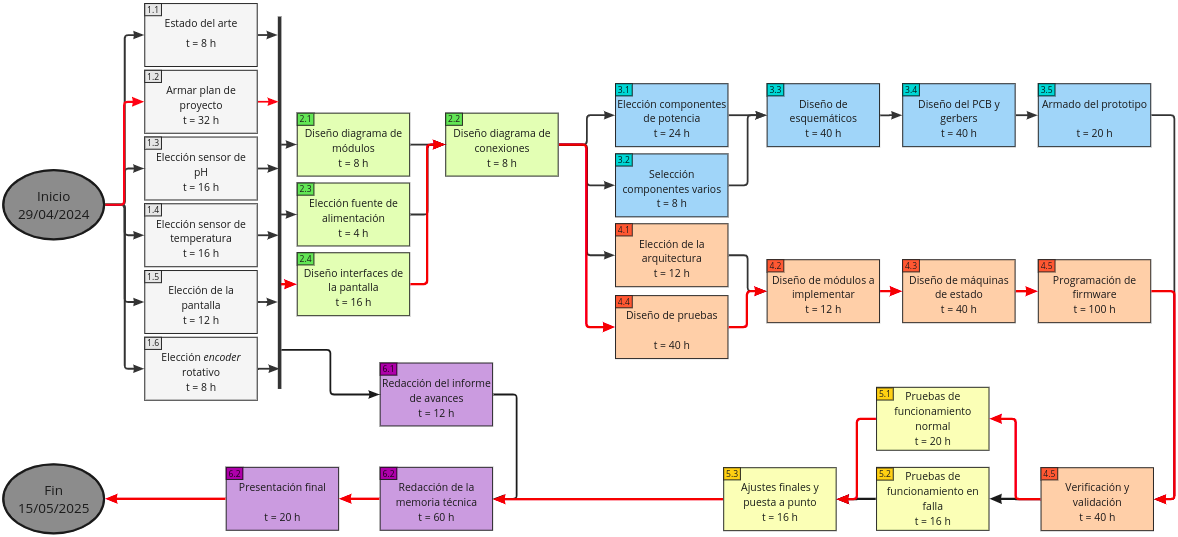
\includegraphics[width=1\textwidth]{./Figuras/AoN-1.png}
\caption{Diagrama de \textit{Activity on Node}.}
\label{fig:AoN}
\end{figure}

\section{11. Diagrama de Gantt}
\label{sec:gantt}

En la figura \ref{fig:gantt-1} y \ref{fig:gantt-2} se muestran el diagrama de Gantt correspondiente a las tareas detalladas en la figura \ref{fig:tasks}. Se toma un calendario de 5 días laborales por semana y se estima un trabajo de 20 horas semanales dividido en 4 horas diarias. Cada 'd' del diagrama representa 4 horas.

\begin{figure}[htpb]
\centering 
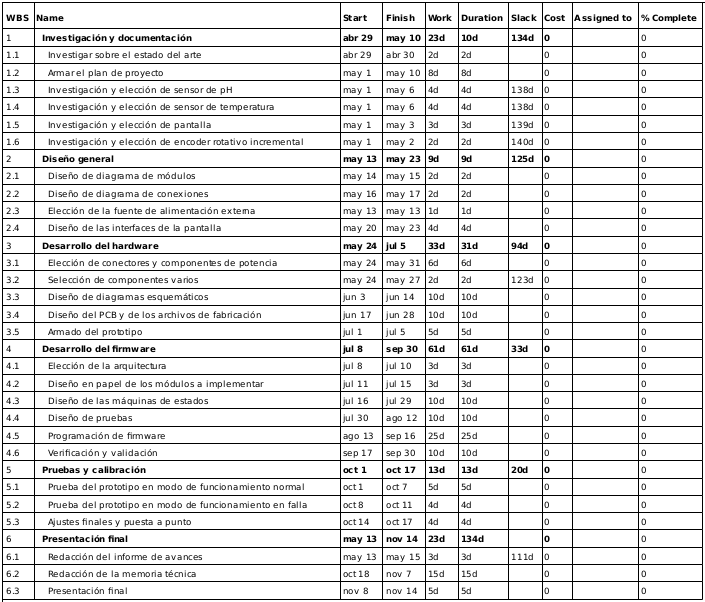
\includegraphics[width=1\textwidth]{./Figuras/tasks.png}
\caption{Tabla de diagrama de Gantt.}
\label{fig:tasks}
\end{figure}

\begin{figure}[htpb]
\centering 
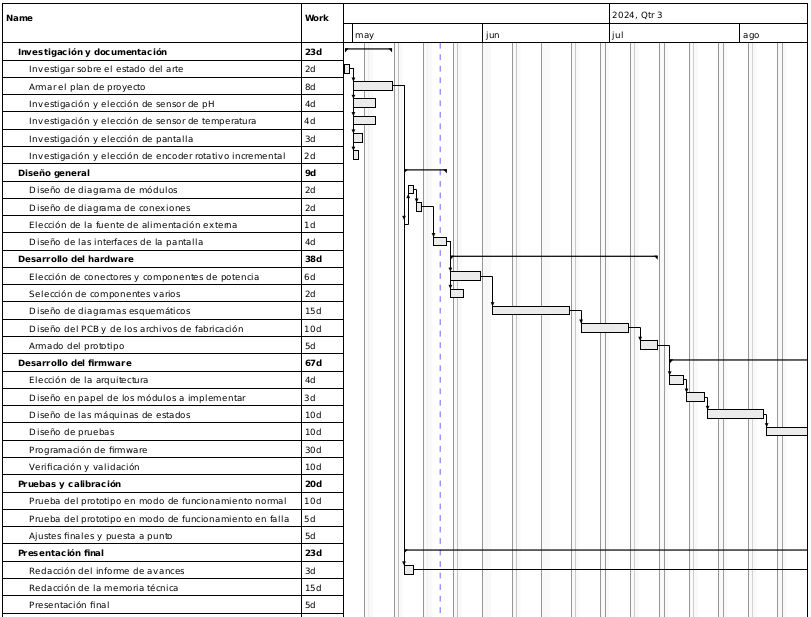
\includegraphics[width=1\textwidth]{./Figuras/gantt-1.png}
\caption{Diagrama de Gantt 1}
\label{fig:gantt-1}
\end{figure}

\begin{figure}[htpb]
\centering 
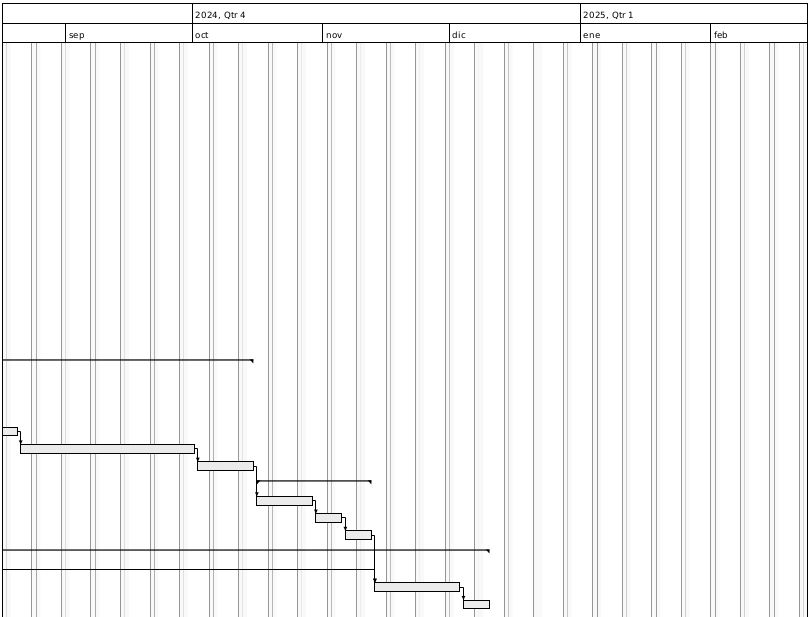
\includegraphics[width=1\textwidth]{./Figuras/gantt-2.png}
\caption{Diagrama de Gantt 2}
\label{fig:gantt-2}
\end{figure}

\section{12. Presupuesto detallado del proyecto}
\label{sec:presupuesto}

Para la siguiente estimación de costos se toma 1 USD = 1000 ARS como tasa de cambio.

\begin{table}[htpb]
\centering
\begin{tabularx}{\linewidth}{@{}|X|c|r|r|@{}}
\hline
\rowcolor[HTML]{C0C0C0} 
\multicolumn{4}{|c|}{\cellcolor[HTML]{C0C0C0}COSTOS DIRECTOS} \\ \hline
\rowcolor[HTML]{C0C0C0} 
Descripción &
  \multicolumn{1}{c|}{\cellcolor[HTML]{C0C0C0}Cantidad} &
  \multicolumn{1}{c|}{\cellcolor[HTML]{C0C0C0}Valor unitario} &
  \multicolumn{1}{c|}{\cellcolor[HTML]{C0C0C0}Valor total} \\ \hline
 
 Salario ingeniero &
  \multicolumn{1}{c|}{ 720 } &
  \multicolumn{1}{c|}{ USD 15 } &
  \multicolumn{1}{c|}{ USD 10800 } \\ \hline
  
 Punta de prueba pH &
  \multicolumn{1}{c|}{ 1 } &
  \multicolumn{1}{c|}{ USD 100 } &
  \multicolumn{1}{c|}{ USD 100 } \\ \hline
  
 Soluciones \textit{buffers} de calibración &
  \multicolumn{1}{c|}{ 3 } &
  \multicolumn{1}{c|}{ USD 10 } &
  \multicolumn{1}{c|}{ USD 30 } \\ \hline
  
 Bomba peristáltica &
  \multicolumn{1}{c|}{ 1 } &
  \multicolumn{1}{c|}{ USD 100 } &
  \multicolumn{1}{c|}{ USD 100 } \\ \hline
  
 Manguera de silicona &
  \multicolumn{1}{c|}{ 1 } &
  \multicolumn{1}{c|}{ USD 20 } &
  \multicolumn{1}{c|}{ USD 20 } \\ \hline

 Sensor de temperatura &
  \multicolumn{1}{c|}{ 1 } &
  \multicolumn{1}{c|}{ USD 50 } &
  \multicolumn{1}{c|}{ USD 50 } \\ \hline
  
 Encoder rotativo con botón &
  \multicolumn{1}{c|}{ 1 } &
  \multicolumn{1}{c|}{ USD 5 } &
  \multicolumn{1}{c|}{ USD 5 } \\ \hline
  
 Fuente de alimentación &
  \multicolumn{1}{c|}{ 1 } &
  \multicolumn{1}{c|}{ USD 10 } &
  \multicolumn{1}{c|}{ USD 10 } \\ \hline   

 Componentes varios para prototipo &
  \multicolumn{1}{c|}{ 1 } &
  \multicolumn{1}{c|}{ USD 50 } &
  \multicolumn{1}{c|}{ USD 50 } \\ \hline  
  
\multicolumn{3}{|c|}{SUBTOTAL} &
  \multicolumn{1}{c|}{ USD 11165 } \\ \hline
  
\rowcolor[HTML]{C0C0C0}
\multicolumn{4}{|c|}{\cellcolor[HTML]{C0C0C0}COSTOS INDIRECTOS} \\ \hline
\rowcolor[HTML]{C0C0C0} 
Descripción &
  \multicolumn{1}{c|}{\cellcolor[HTML]{C0C0C0}Cantidad} &
  \multicolumn{1}{c|}{\cellcolor[HTML]{C0C0C0}Valor unitario} &
  \multicolumn{1}{c|}{\cellcolor[HTML]{C0C0C0}Valor total} \\ \hline
 
\multicolumn{1}{|l|}{30\% del costo directo} &
   \multicolumn{1}{c|}{ 1 } &
   \multicolumn{1}{c|}{ USD 3350 } &
   \multicolumn{1}{c|}{ USD 3350 }\\ \hline
   
\multicolumn{3}{|c|}{SUBTOTAL} &
  \multicolumn{1}{c|}{ USD 3350 } \\ \hline
\rowcolor[HTML]{C0C0C0}
\multicolumn{3}{|c|}{TOTAL} &
   USD 14510\\ \hline
\end{tabularx}%
\end{table}


\section{13. Gestión de riesgos}
\label{sec:riesgos}

\begin{consigna}{red}
a) Identificación de los riesgos (al menos cinco) y estimación de sus consecuencias:
 
Riesgo 1: detallar el riesgo (riesgo es algo que si ocurre altera los planes previstos de forma negativa)
\begin{itemize}
	\item Severidad (S): mientras más severo, más alto es el número (usar números del 1 al 10).\\
	Justificar el motivo por el cual se asigna determinado número de severidad (S).
	\item Probabilidad de ocurrencia (O): mientras más probable, más alto es el número (usar del 1 al 10).\\
	Justificar el motivo por el cual se asigna determinado número de (O). 
\end{itemize}   

Riesgo 2:
\begin{itemize}
	\item Severidad (S): X.\\
	Justificación...
	\item Ocurrencia (O): Y.\\
	Justificación...
\end{itemize}

Riesgo 3:
\begin{itemize}
	\item Severidad (S):  X.\\
	Justificación...
	\item Ocurrencia (O): Y.\\
	Justificación...
\end{itemize}


b) Tabla de gestión de riesgos:      (El RPN se calcula como RPN=SxO)

\begin{table}[htpb]
\centering
\begin{tabularx}{\linewidth}{@{}|X|c|c|c|c|c|c|@{}}
\hline
\rowcolor[HTML]{C0C0C0} 
Riesgo & S & O & RPN & S* & O* & RPN* \\ \hline
       &   &   &     &    &    &      \\ \hline
       &   &   &     &    &    &      \\ \hline
       &   &   &     &    &    &      \\ \hline
       &   &   &     &    &    &      \\ \hline
       &   &   &     &    &    &      \\ \hline
\end{tabularx}%
\end{table}

Criterio adoptado: 

Se tomarán medidas de mitigación en los riesgos cuyos números de RPN sean mayores a...

Nota: los valores marcados con (*) en la tabla corresponden luego de haber aplicado la mitigación.

c) Plan de mitigación de los riesgos que originalmente excedían el RPN máximo establecido:
 
Riesgo 1: plan de mitigación (si por el RPN fuera necesario elaborar un plan de mitigación).
  Nueva asignación de S y O, con su respectiva justificación:
  \begin{itemize}
	\item Severidad (S*): mientras más severo, más alto es el número (usar números del 1 al 10).
          Justificar el motivo por el cual se asigna determinado número de severidad (S).
	\item Probabilidad de ocurrencia (O*): mientras más probable, más alto es el número (usar del 1 al 10).
          Justificar el motivo por el cual se asigna determinado número de (O).
	\end{itemize}

Riesgo 2: plan de mitigación (si por el RPN fuera necesario elaborar un plan de mitigación).
 
Riesgo 3: plan de mitigación (si por el RPN fuera necesario elaborar un plan de mitigación).

\end{consigna}


\section{14. Gestión de la calidad}
\label{sec:calidad}

\begin{consigna}{red}
Elija al menos diez requerimientos que a su criterio sean los más importantes/críticos/que aportan más valor y para cada uno de ellos indique las acciones de verificación y validación que permitan asegurar su cumplimiento.

\begin{itemize} 
\item Req \#1: copiar acá el requerimiento con su correspondiente número.

\begin{itemize}
	\item Verificación para confirmar si se cumplió con lo requerido antes de mostrar el sistema al cliente. Detallar.
	\item Validación con el cliente para confirmar que está de acuerdo en que se cumplió con lo requerido. Detallar. 
\end{itemize}

\end{itemize}

Tener en cuenta que en este contexto se pueden mencionar simulaciones, cálculos, revisión de hojas de datos, consulta con expertos, mediciones, etc.  

Las acciones de verificación suelen considerar al entregable como ``caja blanca'', es decir se conoce en profundidad su funcionamiento interno.  

En cambio, las acciones de validación suelen considerar al entregable como ``caja negra'', es decir, que no se conocen los detalles de su funcionamiento interno.

\end{consigna}

\section{15. Procesos de cierre}    
\label{sec:cierre}

\begin{consigna}{red}
Establecer las pautas de trabajo para realizar una reunión final de evaluación del proyecto, tal que contemple las siguientes actividades:

\begin{itemize}
	\item Pautas de trabajo que se seguirán para analizar si se respetó el Plan de Proyecto original:\\
	 - Indicar quién se ocupará de hacer esto y cuál será el procedimiento a aplicar. 
	\item Identificación de las técnicas y procedimientos útiles e inútiles que se emplearon, los problemas que surgieron y cómo se solucionaron:\\
	 - Indicar quién se ocupará de hacer esto y cuál será el procedimiento para dejar registro.
	\item Indicar quién organizará el acto de agradecimiento a todos los interesados, y en especial al equipo de trabajo y colaboradores:\\
	  - Indicar esto y quién financiará los gastos correspondientes.
\end{itemize}

\end{consigna}

\end{document}